\documentclass[a4paper,12pt]{article}
\usepackage[latin1]{inputenc}
%\usepackage[spanish]{babel}
\usepackage{amssymb}
\usepackage{graphicx}
%\usepackage{textcomp}
\usepackage{geometry}
\geometry{margin=1in}
\usepackage{cite}
\usepackage{url}
\usepackage{hyperref}
\usepackage{float}
\usepackage{amsmath}
\usepackage{cleveref}

\crefformat{footnote}{#2\footnotemark[#1]#3}

\title{\textbf{Project 2: Classical Planning}}
\author{Miguel Tasende}

%opening
\begin{document}


\maketitle

\section{Introduction}
This report shows the results of solving some ``Air Cargo'' (logistics planning) problems with different search algorithms (on top of a graph plan).

\section{Problems 1 and 2}
The first two problems were solved using each of the search algorithms. The results can be seen on the table below.

\begin{figure}[!h]
\centering
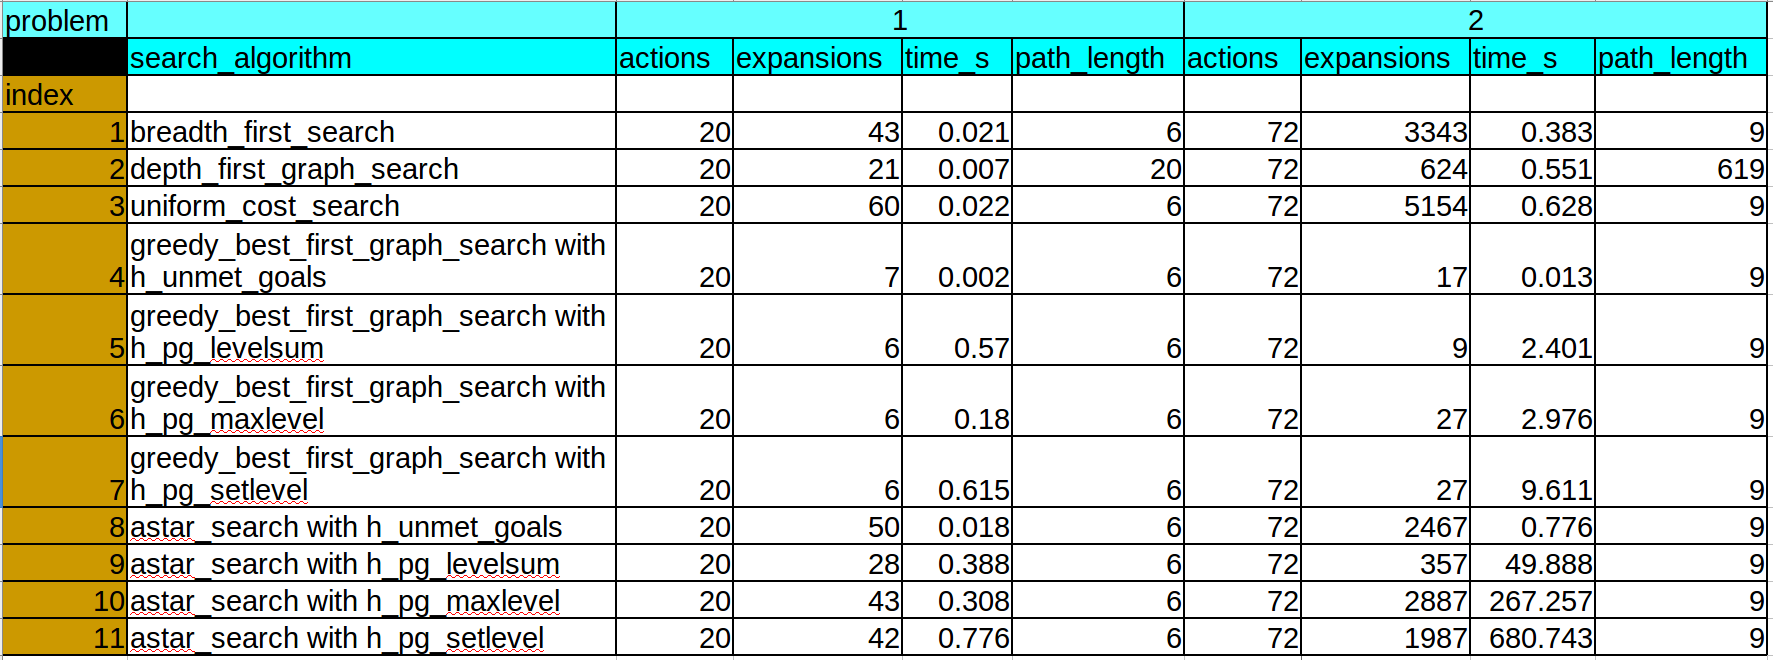
\includegraphics[width=6.0in]{results/results12.png}
\caption{Results for the first two problems, with all the search algorithms}
\label{fig_raw_data}
\end{figure}

It was noticed that the Depth First algorithm was resulting in extremely long paths, and considering this is an Air Cargo problem, it is reasonable to expect that optimum or near-optimum solutions are searched for. Therefore, the Depth First algorithm won't be considered in the rest of the project.\\
$A^*$ with ``maxlevel'' and ``setlevel'' heuristics are taking a lot of time to find a solution, but they will be considered for the other problems, to have more data (it is expected that running all the remaining combinations may take about 10 hours of processing with pypy3).

\section{Problems 3 and 4}
Problems 3 and 4 were solved with all the algorithms except Depth First. In the case of Problem 4, the A* algorithm with the ``project goals set level'' heuristic didin't finish in a reasonable time, and so it was stopped. The results are below.

\begin{figure}[!h]
\centering
\includegraphics[width=6.0in]{results/results34.png}
\caption{Results for the last two problems}
\label{fig_raw_data}
\end{figure}

\newpage
\section{Aggregated Results}
Some tables and charts are shown below, aggregating the results for all problems, and all search algorithms in different ways.

\subsection{Number of expanded nodes}
\begin{figure}[!h]
\centering
\includegraphics[width=4.0in]{results/table_expansions_actions.png}
\caption{Table showing the number of expanded nodes against the number of actions for each algorithm.}
\label{fig_raw_data}
\end{figure}

\begin{figure}[!h]
\centering
\includegraphics[width=6.5in]{results/expansions_actions.png}
\caption{Chart showing the number of expanded nodes against the number of actions for each algorithm. The y-axis scale is logarithmic.}
\label{fig_raw_data}
\end{figure}

The growth of the expanded nodes is exponential ($C e^{\alpha a}$) for all the algorithms, but each one has a different $\alpha$ and $C$.

\newpage
\subsection{Time to complete the search}
\begin{figure}[!h]
\centering
\includegraphics[width=4.0in]{results/table_time_actions.png}
\caption{Table showing the time to complete the search (in seconds) against the number of actions for each algorithm.}
\label{fig_raw_data}
\end{figure}

\begin{figure}[!h]
\centering
\includegraphics[width=6.5in]{results/time_actions.png}
\caption{Chart showing the time to complete the search (in seconds) against the number of actions for each algorithm. The y-axis scale is logarithmic.}
\label{fig_raw_data}
\end{figure}

The growth of the search time is exponential ($C e^{\alpha a}$) for all the algorithms, but each one has a different $\alpha$ and $C$.

\newpage
\subsection{Length of the plan for each problem}
\begin{figure}[!h]
\centering
\includegraphics[width=4.0in]{results/table_length_problem.png}
\caption{Length of the resulting plan for each problem and each algorithm.}
\label{fig_raw_data}
\end{figure}

\begin{figure}[!h]
\centering
\includegraphics[width=6.5in]{results/length_problem.png}
\caption{Length of the resulting plan for each problem and each algorithm.}
\label{fig_raw_data}
\end{figure}

It can be readily seen that many of the algorithms aren't optimal. Except the case of Depth First Search, the others are ``not so far away'' from the optimal solution. The algorithm ids references can be seen below (the x-axis was too small to use the entire names):
\begin{figure}[!h]
\centering
\includegraphics[width=3.0in]{results/references.png}
\caption{Algorithm ids references.}
\label{fig_raw_data}
\end{figure}


\newpage
\section{Results Analysis}
\subsection{Which algorithm or algorithms would be most appropriate for planning in a very restricted domain (i.e., one that has only a few actions) and needs to operate in real time?}
The answer would depend on the precise meaning of ``real time'' and ``a few actions''. Assuming that a sub-second response is desired and that there are about 20 to 70 actions, I would choose Breadth First Search, because it guarantees optimality, it can comply with the time restrictions, and it is very simple. If the ``real time'' condition is more restrictive, one could use Greedy Best First Graph Search with the ``unmet goals'' heuristic. That won't guarantee the optimality but it will be extremely fast (tens of milliseconds, less than the blink of an eye [that takes about 250ms]). Uniform Cost Search would be acceptable in some cases, but it offers no advantage to Breadth First Search.


\subsection{Which algorithm or algorithms would be most appropriate for planning in very large domains (e.g., planning delivery routes for all UPS drivers in the U.S. on a given day)}
A complete cost-benefit analysis may reveal that it may be worth dedicating more computing resources, or software optimization efforts to getting better results, but I will answer considering my laptop performance with the current algorithms... In that case, if there are some tens of thousands of UPS drivers, the only algorithm that seems to be able to cope with the problem, in a reasonable time [less than 12 hours, assuming the planning is done in the night before, for example], is Greedy Best First Graph Search with the ``unmet goals'' heuristic. It doesn't guarantee optimality of the path, but the experimental lengths in the assignment were not so bad. The second choice would be A* with the ``unmet goals'' heuristic (doesn't guarantee optimality, and takes longer time, but may get closer-to-optimal results, in some cases)


\subsection{Which algorithm or algorithms would be most appropriate for planning problems where it is important to find only optimal plans? }
Breadth First Search, Uniform Cost Search, A* with the ``problem goals maxlevel'' heuristic, or A* with the ``problem goals setlevel'' heuristic. None of the greedy algorithms can guarantee optimality of the path, nor can Depth First Search. The ``unmet goals'' and ``level sum'' heuristics are not admissible, and so they can't be used if optimality is needed.


\end{document}